\documentclass{coursclass}

\usepackage{xfp}

\newgeometry{
	bottom=0.7cm,
	top=0.7cm,
	left=1.5cm,
	right=1.5cm
}

\title{}
\author{}
\date{}

\begin{document}
\thispagestyle{plain}

\newcommand{\computef}[1]{
	\fpeval{-0.1*#1*#1 + 0.5*#1 + 2}%
}
\newcommand{\repereXLow}{-5.5}
\newcommand{\repereXHigh}{5.5}
\newcommand{\repereYLow}{-3.5}
\newcommand{\repereYHigh}{3.5}
\newcommand{\Exemple}{
	\begin{exemple}
		Soit $f$ une fonction, dont le graphe est donné ci-dessous :

		\begin{center}
			\begin{tikzpicture}[scale=0.7]
				\draw[thin,gray] (\repereXLow,\repereYLow) grid (\repereXHigh,\repereYHigh);
				\draw[thick,\myArrow] (\repereXLow,0) -- (\repereXHigh,0) node[below right] {$x$};
				\draw[thick,\myArrow] (0,\repereYLow) -- (0,\repereYHigh) node[above left] {$y$};

				\draw[orange,ultra thick,domain=\repereXLow+0.5:\repereXHigh-0.5,variable=\x] plot({\x},{-0.1*\x*\x + 0.5*\x + 2}) node[above] {$𝒞_f$};

				\newcommand{\A}{-2.6234753829797994}
				\newcommand{\B}{2.5}

				\draw[blue,dashed] (-5,-0.2) node[below] {$-5$} -- (-5,-3) -- (0.2,-3) node[right] {$-3$};
				\draw[blue,dashed] (\A,0) -- ++(0,-0.2) node[below] {$-2,6$} -- (\A,\computef{\A});
				\draw[blue,dashed] (\B,0) -- ++(0,-0.2) node[below] {$2,5$} -- (\B,\computef{\B}) -- (-0.2,\computef{\B}) node[left] {$2,7$};
				\draw[blue,dashed] (5,-0.2) node[below] {$5$} -- (5,2) -- (-0.2,2) node[left] {$2$};
			\end{tikzpicture}
		\end{center}

		Le tableau de signes de $f$ est :

		\begin{center}
			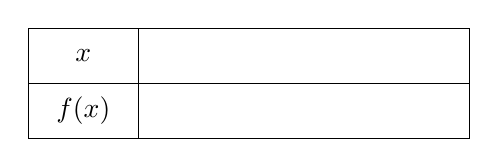
\begin{tikzpicture}[scale=0.7]
				\draw (0,0) -- ++(8,0) -- ++(0,-2) -- ++(-8,0) -- cycle;
				\draw (0,-1) -- ++(8,0);
				\draw (2,0) -- ++(0,-2);

				\node at (1,-0.5) {$x$};
				\ifdefined\makeCorrection
					\node[red] at (2.6,-0.5) {$-5$};
					\node[red] at (5,-0.5) {$-2,6$};
					\node[red] at (7.4,-0.5) {$5$};
				\fi

				\node at (1,-1.5) {$f(x)$};
				\ifdefined\makeCorrection
					\node[red] at (3.5,-1.5) {$-$};
					\node[red] at (5,-1.5) {$0$};
					\node[red] at (6.5,-1.5) {$+$};
					\draw[red] (5,-1) -- ++(0,-0.25) ++ (0,-0.5) -- ++(0,-0.25);
				\fi
			\end{tikzpicture}
		\end{center}

		Le tableau de variations de $f$ est :

		\begin{center}
			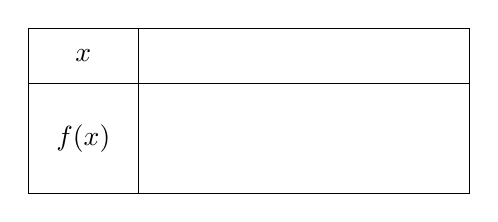
\begin{tikzpicture}[scale=0.7]
				\draw (0,0) -- ++(8,0) -- ++(0,-3) -- ++(-8,0) -- cycle;
				\draw (0,-1) -- ++(8,0);
				\draw (2,0) -- ++(0,-3);

				\node at (1,-0.5) {$x$};
				\ifdefined\makeCorrection
					\node[red] at (3,-0.5) {$-5$};
					\node[red] at (5,-0.5) {$2,5$};
					\node[red] at (7,-0.5) {$5$};
				\fi

				\node at (1,-2) {$f(x)$};
				\ifdefined\makeCorrection
					\node[red] at (3,-2.5) {$-3$};
					\node[red] at (5,-1.5) {$2,7$};
					\node[red] at (7,-2.5) {$2$};

					\draw[red,->] (3.3,-2.3) -- (4.6,-1.7);
					\draw[red,->] (5.3,-1.7) -- (6.6,-2.3);
				\fi
			\end{tikzpicture}
		\end{center}
	\end{exemple}
}

\Exemple

\vspace{0.6cm}

\Exemple

\end{document}